\documentclass[../mainV8.tex]{subfiles}
%\graphicspath{{\subfix{../images/}}}
\usetikzlibrary{positioning}
\begin{document}


% \documentclass[tikz]{standalone}
% \usetikzlibrary{positioning}

%\begin{document}
\begin{figure}[h]
\centering

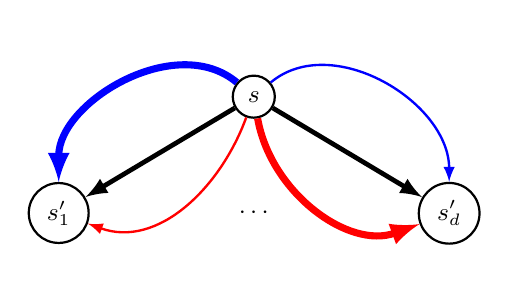
\begin{tikzpicture}[auto, node distance=8mm, >=latex, font=\small]
    % Define node styles
    \tikzstyle{round} = [thick, draw=black, circle]
    
    % Nodes
    \node[round] (s0) {$s$};
    
    \node[round, below left=10mm and 20mm of s0] (s1) {$s'_1$};
    %%%
    \node[below=10mm of s0] (s2) {$\cdots$};
    %%%
    \node[round, below right=10mm and 20mm of s0] (s3) {$s'_d$};
%%%%%%%%%%%%%%%
%%%%%%%%%%%%%%%%%%%%%%%%%%%%%%
%%%%%%%%%%%%%%%
%transitions
% %      \draw[->, black, thick, , line width=0.5mm] (s0) to[out=100, in=140,, line width=0.5mm] (s1);  % the black one on the top
% %     %%%
% %       \draw[->, black, ultra thick,, line width=0.5mm] (s0) to[out=-45, in=135] (s3);
% % %%%%%%%%%%%%%%%
% % %%%%%%%%%%%%%%%
% %     \draw[->, blue, very thick,, line width=0.7mm] (s0) to[out=80, in=160] (s1); 
% %     % the blue one on the top
% %     \draw[->, blue, very thick, , line width=0.3mm] (s0) to[out=-60, in=195] (s3); 
% %%%%%%%%%%%%%%%
% %%%%%%%%%%%%%%%
%      \draw[->,  red, ultra thick, line width=0.3mm] (s0) to[out=45, in=190] (s1);
%      % the red one on the top
%     \draw[->, red, thick, , line width=0.7mm] (s0) to[out=-45, in=180,] (s3); 


% Direct line
    \draw[->, black, thick,line width=0.6mm] (s0) -- (s1);

    % First arched line
    \draw[->, blue, thick, line width=0.9mm] (s0) to[out=140, in=90] (s1);

    % Second arched line
    \draw[->, red, thick,line width=0.3mm] (s0) to[out=250, in=-20] (s1);



    \draw[->, blue, thick,line width=0.3mm] (s0) to[out=40, in=90] (s3);
    % Direct line
    \draw[->, black, thick,line width=0.6mm] (s0) -- (s3);
    % First arched line
    \draw[->, red, thick,line width=0.9mm] (s0) to[out=-80, in=-160] (s3);
\end{tikzpicture}


\caption{A learner at  $s$  selects a color and transitions to  $S^{\prime}$. Each color represents a probability vector, meaning that the likelihood of arriving at a destination varies depending on the chosen color.}
\label{fig:systemmodel}
\end{figure}
\end{document}